\chapter{Sistema Desenvolvido}
\label{chap:sistema-desenvolvido}

Como exposto no Capítulo \ref{chap:dispositivos-protocolos}, são necessários vários protocolos ou adaptações para que a comunicação de um processo consiga atingir interoperabilidade entre o servidor e todos os dispositivos. Os sistemas \gls{SCADA} demonstrados no Capítulo \ref{chap:scada} utilizados para receber estas informações do servidor \gls{OPC} local ou diretamente destes dispositivos e organizá-las em um banco de dados, é a forma predominante na indústria e a forma mais confiável hoje. Todos os \textit{softwares} disponíveis para utilização que foram citados têm em comum seu modo de funcionamento, onde é instalado em uma máquina próxima e fisicamente ligada ao processo, que por sua vez mantém todos os serviços necessários para o funcionamento integrado dos módulos que o compõe. Alguns dispõem de integração com o protocolo \gls{MQTT} e interfaceamento \gls{WEB}, mas não são nativamente desenvolvidos para o funcionamento remoto.

Este trabalho propõe o desenvolvimento de um sistema \gls{SCADA} \gls{WEB} em que sua distribuição não seja mais como os sistemas \gls{SCADA} citados, na forma de um Produto como Serviço onde o cliente paga por um \textit{software} desenvolvido e futuras atualizações que venham ocorrer mas fornece toda a estrutura necessária para o funcionamento dele, e sim \textit{Software} como Serviço, do inglês, \gls{SaaS}, em que a própria plataforma fornece os recursos necessários para a disponibilização de todos os módulos do sistema, sejam eles: servidores, segurança e atualizações do próprio \textit{software}.

Com a premissa de que toda a estrutura esteja disponível através da \textit{internet}, além de todas as funcionalidades de um sistema \gls{SCADA} convencional, várias vantagens podem ser listadas como:

\begin{alineascomponto}
    \item a capacitação profissional que antes seria necessária para a operação dessa estrutura é extremamente simplificada ao manuseio da interface;
    \item o gerenciamento é feito exclusivamente através do navegador podendo ser utilizado por todas as plataformas existentes na empresa, desde computadores, à \textit{smartphones} e \textit{tablets};
    \item com o uso da computação em nuvem, é possível a escalabilidade de recursos, sejam eles armazenamento ou processamento e tarefas simples que demandariam mais servidores ou a parada da aquisição de dados, podem agora ser feitas diretamente pela plataforma sem haver prejuízos ao processo;
    \item o mesmo sistema pode gerenciar múltiplos processos utilizando a mesma estrutura, podendo serem ou não apresentados na mesma interface;
    \item envio e recebimento de dados do processo podem ser feitos diretamente pelos dispositivos citados no Capítulo \ref{chap:dispositivos-protocolos} para a plataforma remota, desde que estejam disponíveis estas funcionalidades;
    \item com a possibilidade de uso de \gls{API} \gls{HTTP}, outros sistemas utilizados pela empresa podem trabalhar diretamente com o sistema \gls{SCADA}, obtendo informações ou atuando sobre o processo, se necessário e desejado.
\end{alineascomponto}

Algumas desvantagens também são conhecidas inicialmente devido seu modo de funcionamento, como:

\begin{alineascomponto}
    \item existência de um tempo de atraso na casa de milisegundos entre o envio e o recebimento das informações entre servidor e cliente devido a estrutura ser concebida de forma remota, relativamente longe do processo ao que seria a estrutura convencional;
    \item a dependência de uma boa conexão com a \textit{internet} e estabilidade desta para a utilização do sistema, que pode ser amenizada caso os dispositivos utilizados tenham uma memória local capaz de armazenar os dados no caso de uma queda na conexão por uma janela de tempo suficiente até o retorno desta;
    \item dispositivos que não tenham nativamente acesso à \textit{internet} deverão contar com drivers de comunicação capazes de intermediar estas informações ao sistema, como já acontece no \gls{SCADA} tradicional.

\end{alineascomponto}

\section{Projetos}
\label{sec:projetos}
No sistema \gls{SCADA} proposto, são definidos alguns conceitos:

\begin{alineascomponto}
    \item Variável: Um conjunto de informações enviadas pelos dispositivos do processo ao módulo de aquisição de dados, que criam uma linha temporal no banco de dados do sistema.
    \item Objetos: Caixas para conteúdo visual, que utilizarão as informações contidas nas Variáveis para apresentá-las por gráficos, tabelas, texto estático ou permitir a interação com o processo através de chaves, botões ou outros recursos.
    \item Projeto: Estrutura lógica ao qual serão organizados Objetos de forma intuitiva na interface \gls{WEB} para compor todas as informações necessárias para apresentação do processo trabalhado.
    \item Desenvolvedor do Projeto: Usuário principal do Projeto que possua permissão de inserção ou manutenção da organização de Objetos, gerenciamento de Variáveis e outras funções mais restritas.
    \item Operador: Usuário com permissão apenas de visualizar as informações e/ou interagir com o processo através de chaves, botões e outros recursos.
\end{alineascomponto}

O sistema permite a criação ou visualização de múltiplos Projetos na mesma conta de forma totalmente isolada, baseado no exemplo de indústrias que dependam de mais de um processo ou tenham setores bem definidos que necessitem de interfaces de gerenciamento diferentes. Para que um novo Projeto seja constituído, o Desenvolvedor do Projeto o insere na plataforma através da interface de gerenciamento, cadastra variáveis relativas ao processo considerando seus tipos e em seguida cria novos Objetos necessários, cada Objeto poderá ter associado uma ou mais variáveis, para que o conteúdo destas ganhem forma, seja em forma de gráficos, tabelas ou para permitir o interação e controle do processo à um Operador. Estes objetos possuem configuração específica ao seu tipo, como o o tamanho da janela de tempo que serão mostradas as informações por exemplo, mais detalhes serão dados à frente. Após toda a organização do Projeto, o Desenvolvedor do Projeto pode cadastrar os Operadores que irão monitorar e operar a interface de gerenciamento. A Figura \ref{fig:figura-projetos} traz um esquemático de como seria a hierarquia desses elementos em relação ao Projeto. 

        \begin{figure}[!h]
		\Caption{\label{fig:figura-projetos} Lógica e hierarquia dos projetos desenvolvidos no sistema.}
		%\centering
		\UFCfig{}{
			\fbox{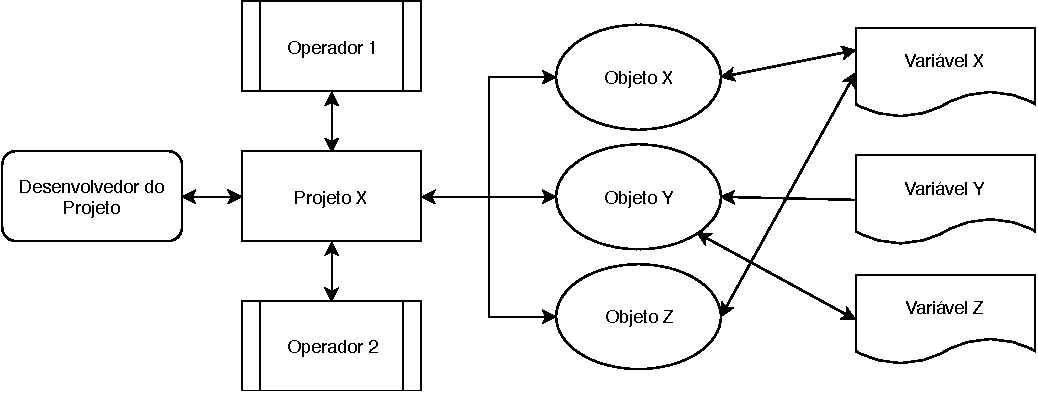
\includegraphics[width=15cm]{figuras/projetos.pdf}}
		}{
			\Fonte{O autor}
		}	
    	\end{figure}

    \section{Armazenamento dos Dados}
    \label{sec:armazenamento-dados}
    
    Os dados enviados para a plataforma, serão tratados e inseridos em um banco de dados relacional, contendo chave e valor, onde é dada para o usuário uma ideia de variável de programação para a chave. Também, são descritos tipos de variáveis em que sua utilização serão considerados, como exemplo de uma chave liga/desliga que poderá utilizar uma variável binária. Mais detalhes sobre os tipos de variável e o banco de dados utilizado são dados abaixo.
    
        \subsection{Tipos de Variáveis}
        \label{sec:tipos-variaveis}
            
        \begin{alineascomponto}
            \item Binária: conhecida também por variável booleana, são permitidos valores 0 ou 1, false ou true e, dentro da plataforma, utilizada para chaves liga/desliga ou botões;
            \item Numérica: valores numéricos inteiros ou racionais, positivos ou negativos, que não ultrapassem o valor de 15 algarismos significativos ou 3 casas decimais;
            \item Texto: similar à variável \textit{string} de linguagens de programação, onde pode assumir qualquer valor com um tamanho máximo de 254 posições de texto.
        \end{alineascomponto}
        
        \subsection{Banco de Dados}
        \label{sec:banco-dados}
        O banco de dados utilizado para este projeto foi o \textit{software} MariaDB, desenvolvido pela MariaDB Foundation, é um dos projetos de bancos de dados mais populares do mundo, possui código aberto baseado no \textit{MySQL} e, por ser um banco relacional, seu uso é feito através de Linguagem de Consulta Estruturada, do inglês, \gls{SQL}, possuindo suporte para os tipos de dados mais comuns. É utilizado por grandes empresas, como: Wikipedia, Google, Booking.com, Alibaba.com e Microsoft \cite{MariaDB}. A Figura \ref{fig:figura-mqtt-servico} mostra o logotipo do projeto utilizado.
        
        \begin{figure}[!h]
		\Caption{\label{fig:figura-mariadb-servico} Projeto de banco de dados de código aberto MariaDB.}
		%\centering
		\UFCfig{}{
			\fbox{
\includegraphics[width=5cm]{figuras/mariadb.png}}
		}{
			\Fonte{\cite{MariaDB}}
		}	
    	\end{figure}
    	
\section{Aquisição de Dados}
\label{sec:aquisicao-dados}
O módulo mais importante para o funcionamento deste sistema é a aquisição de dados, pois através deles se dará o direcionamento de todos os outros módulos. Conforme descritos no Capítulo \ref{chap:dispositivos-protocolos}, os protocolos \gls{HTTP} e \gls{MQTT} são  projetados para \gls{WEB} e possuem compatibilidade com diversos formatos de dados, sendo este o motivo para escolha deles neste projeto. Será feita uma abstração da camada física de dispositivos que utilizem \gls{OPC} por exemplo, partindo do pressuposto que estes possuam drivers de comunicação que possam fazer envio destes dados pela \textit{internet}, ou seja, não haverá discriminação sobre os dados recebidos e tratados na plataforma. O utilizador da plataforma poderá escolher entre os dois protocolos de acordo com sua aplicação de interesse, abaixo são detalhados os processos referentes à aquisição de dados de cada um deles.

        \subsection{HTTP}
        \label{sec:aquisicao-http}
        O protocolo \gls{HTTP} será utilizado para a construção de uma \gls{API} baseada em \gls{REST} que possua a maior compatibilidade possível entre os métodos de chamada, para que até dispositivos simples possam trocar informações mesmo utilizando métodos de chamada triviais. Serão aceitos aqui, os três formatos de conteúdo descritos na seção \ref{sec:formatos-de-conteudo} devido o suporte nativo deste protocolo.
        
        Basicamente o processo de envio ou gerenciamento das informações contidas na plataforma, serão organizadas em 4 etapas: (i) Validação das Informações, (ii) Autenticação, (iii) Identificação das Informações, (iv) Banco de Dados, que serão detalhadas individualmente adiante. A Figura \ref{fig:figura-http-geral} traz um diagrama representando a sequência lógica destas quando iniciada a requisição.
        
        \begin{figure}[!h]
		\Caption{\label{fig:figura-http-geral} Diagrama das etapas do servidor para manipulação de dados.}
		%\centering
		\UFCfig{}{
			\fbox{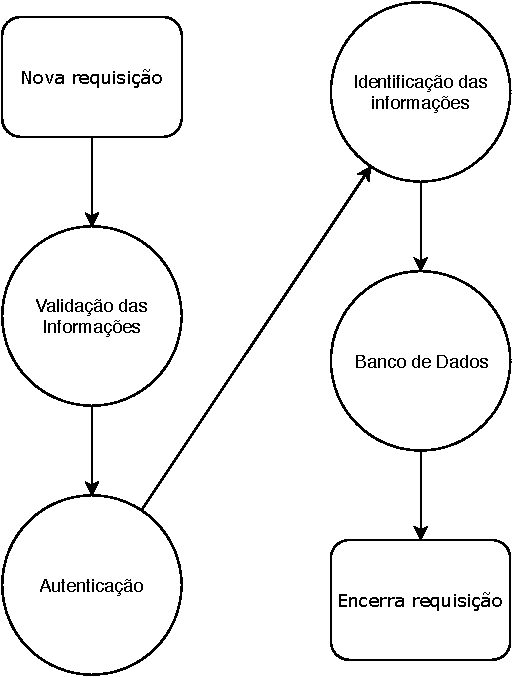
\includegraphics[width=8cm]{figuras/http-geral.pdf}}
		}{
			\Fonte{O autor}
		}	
    	\end{figure}
    	
    	\begin{figure}[!h]
		\Caption{\label{fig:figura-http-validacao} Diagrama de validação das informações recebidas.}
		%\centering
		\UFCfig{}{
			\fbox{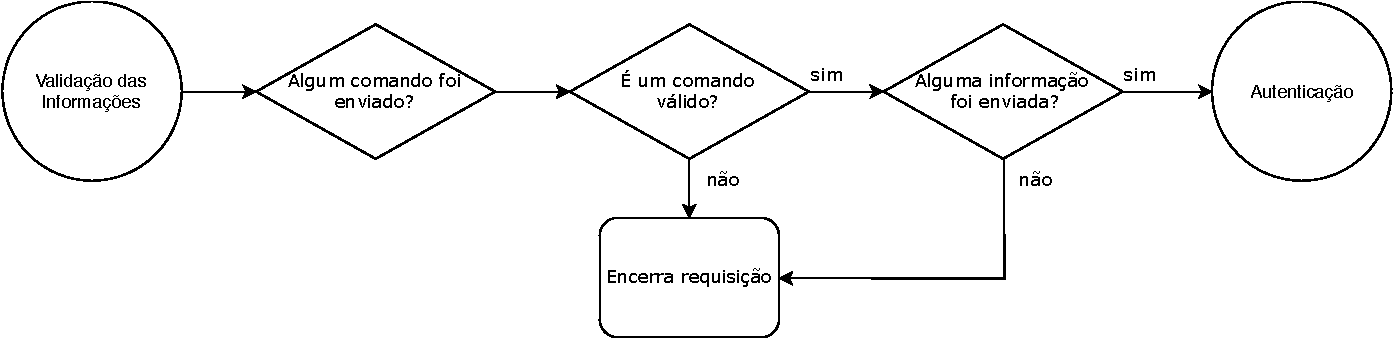
\includegraphics[width=15cm]{figuras/http-validacao.pdf}}
		}{
			\Fonte{O autor}
		}	
    	\end{figure}
    	
    	 Através de parâmetros configurados na \gls{URL} da \gls{API} da plataforma e cabeçalhos da requisição, o módulo identifica o método de chamada e qual comando o utilizador deseja. Se o comando enviado for reconhecido pelo módulo e exista alguma informação válida à ser enviada, é dado o direcionamento à etapa seguinte da Autenticação, caso contrário, a requisição é imediatamente encerrada. A Figura \ref{fig:figura-http-validacao} traz um diagrama com detalhes da etapa de validação das informações.
    	 
    	 Posteriormente, dentre os parâmetros enviados é feita uma verificação do \textit{token}, um código que funciona como uma senha e, caso seja válido e esteja autorizado ao uso da \gls{API}, o módulo verifica seu limite de envios no caso de novas inserções de informações e segue à próxima etapa caso esteja apto, encerrando a requisição caso contrário. A Figura \ref{fig:figura-http-autenticacao} traz um diagrama detalhando a lógica da autenticação.
    	
    	\begin{figure}[!h]
		\Caption{\label{fig:figura-http-autenticacao} Diagrama de autenticação do usuário.}
		%\centering
		\UFCfig{}{
			\fbox{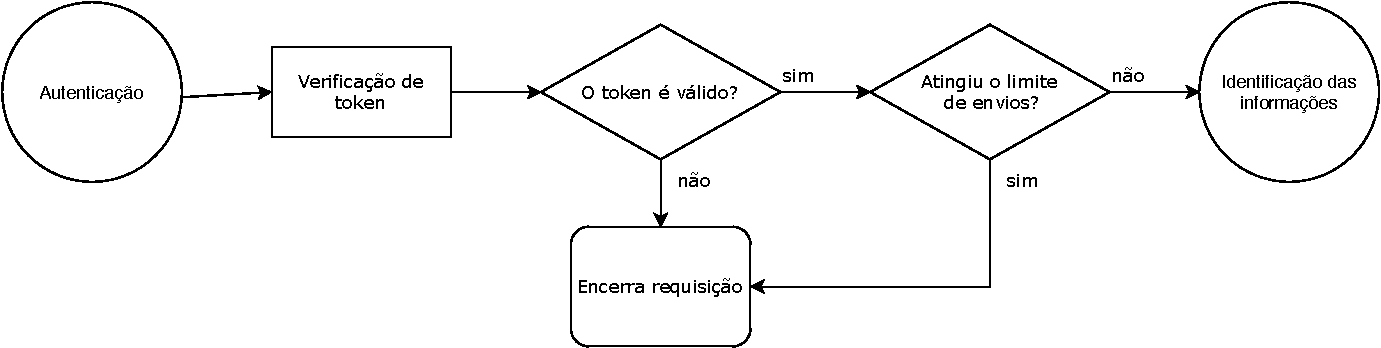
\includegraphics[width=15cm]{figuras/http-autenticacao.pdf}}
		}{
			\Fonte{O autor}
		}	
    	\end{figure}
    	
    	 Na etapa de Identificação do tipo de informação enviada, basicamente são listadas todas as variáveis que se deseja inserir ou modificar no banco de dados e a categorização delas, sejam: númericas, binárias ou texto. A Figura \ref{fig:figura-http-identificacao} traz detalhes sobre a identificação das informações provenientes da requisição.
    	
    	\begin{figure}[!h]
		\Caption{\label{fig:figura-http-identificacao} Diagrama sobre a identificação do tipo das informações.}
		%\centering
		\UFCfig{}{
			\fbox{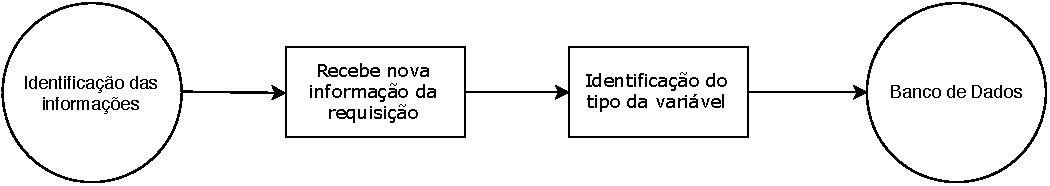
\includegraphics[width=15cm]{figuras/http-identificacao.pdf}}
		}{
			\Fonte{O autor}
		}	
    	\end{figure}
    	
    	Por último, são verificadas uma a uma se o nome das variáveis já estão cadastradas no banco de dados e é dado o direcionamento para elas, repetindo a etapa de identificação para cada informação enviada, encerrando a requisição após o tratamento de todas elas. A Figura \ref{fig:figura-http-banco} traz mais detalhes sobre a etapa do banco de dados.
    	
    	\begin{figure}[!h]
		\Caption{\label{fig:figura-http-banco} Diagrama da etapa de banco de dados.}
		%\centering
		\UFCfig{}{
			\fbox{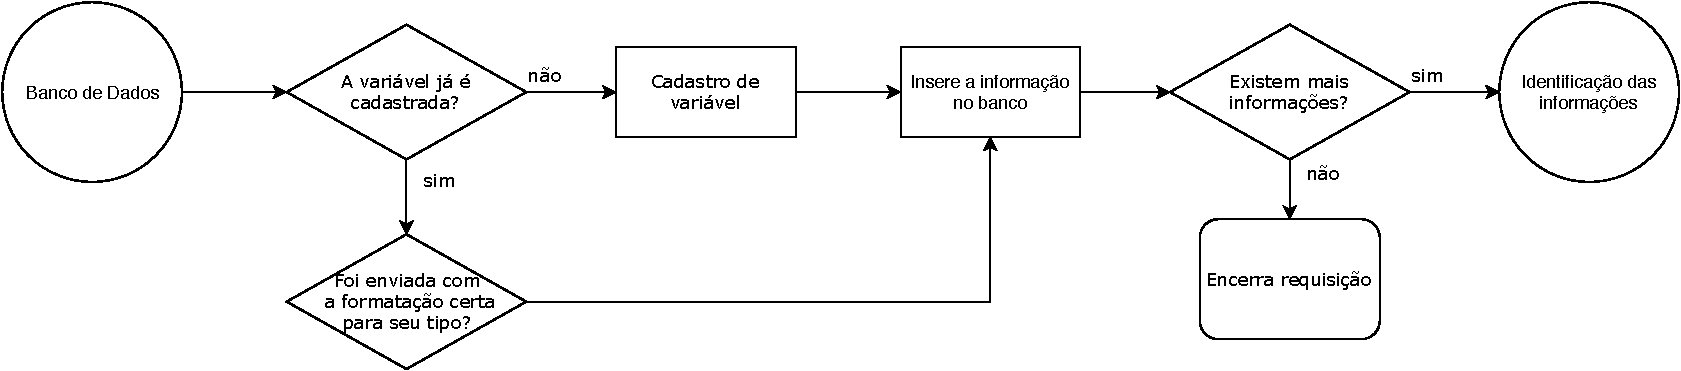
\includegraphics[width=15cm]{figuras/http-banco.pdf}}
		}{
			\Fonte{O autor}
		}	
    	\end{figure}
        
        \subsection{MQTT}
        \label{sec:aquisicao-mqtt}
        O protocolo \gls{MQTT} será utilizado para o envio e recebimento de informações de dispositivos que tenham restrição de largura de banda ou que tenham suporte nativo à sua utilização, devido sua facilidade de uso. Se faz necessária uma aplicação \textit{broker} para o funcionamento deste serviço e, devido ser um projeto de código aberto, foi escolhido o \textit{software} VerneMQ para esta finalidade. O projeto foi desenvolvido para ser distribuído, ou seja, há a possibilidade de escalabilidade vertical (quando se inclui mais servidores para a manutenção do serviço) e horizontal (quando se aumenta os recursos de um único servidor), em conformidade com o avanço da utilização crescente deste protocolo com a introdução da \textit{internet} das coisas. Além disto, traz funcionalidades como: autenticação, criptografia, níveis de serviço, envio de mensagens \textit{offline}, balanceamento de recursos, entre outros \cite{VerneMQ}. A Figura \ref{fig:figura-mqtt-servico} mostra o logotipo do serviço utilizado e as principais plataformas suportadas.
        
        \begin{figure}[!h]
		\Caption{\label{fig:figura-mqtt-servico} Projeto utilizado para manter o serviço do MQTT.}
		%\centering
		\UFCfig{}{
			\fbox{
\includegraphics[width=10cm]{figuras/vernemq.png}}
		}{
			\Fonte{Adaptado de \cite{VerneMQ}}
		}	
    	\end{figure}
    	
    	Conforme explicado na seção \ref{sec:mqtt}, o MQTT recebe e envia informações através de tópicos e, no caso desta plataforma, para o envio de informações, são considerados: tópico como o \textit{token} do usuário e sub-tópico como a variável cadastrada no projeto em que se deseja inserir no banco de dados, simplificando portanto a autenticação deste serviço e tornando similar ao uso da \gls{API} \gls{HTTP}. O módulo de aquisição de dados para o MQTT funciona como um subscritor neste serviço, capturando as informações enviadas pelo usuário no \textit{broker} e inserindo-as no banco de dados caso sejam válidas, o retorno de informação é dado pelo mesmo canal de envio. Os níveis de qualidade de serviço para a entrega das mensagens podem ser utilizados à critério de projeto pelo usuário.

\section{Segurança}
    \label{sec:seguranca}
    Além do \textit{token} citado na seção \ref{sec:aquisicao-dados}, outros elementos e critérios de segurança são considerados para garantir a segurança dos dados manipulados dentro da plataforma, todos os critérios de segurança desenvolvidos neste projeto serão detalhados nas seções abaixo.
        
        \subsection{Criptografia}
        \label{sec:criptografia}
        Por se tratar de dados críticos e de potencial de interesse comercial do cliente, optou-se pela implementação de criptografia ponta a ponta não somente na área de acesso da interface de gerenciamento, mas também no módulo de aquisição de dados, ficando a critério do cliente a sua utilização ou não, já que podem ser incrementados um pequeno atraso de tempo e recursos na sua utilização, perceptíveis em processos que necessitem de curtos intervalos de tempo para funcionamento.  Em ambos os módulos, gerenciamento e aquisição de dados, é utilizado o protocolo \gls{HTTPS} visto na seção \ref{sec:https}, que utiliza certificados fornecidos por autoridades de certificação, como exemplo a empresa \textit{VeriSign} entre outras que são autorizados previamente nos navegadores, tendo a certeza de uma conexão segura e autêntica é implementada a criptografia \gls{TLS} entre servidor e cliente e a requisição é concluída similarmente ao que seria no protocolo \gls{HTTP} comum, o mesmo acontece para o protocolo \gls{MQTT} quando necessária sua utilização.
        
        \subsection{Proteções}
        \label{sec:protecoes}
        
        Alguns métodos são implementados para garantir que não haja vazamento ou quaisquer problemas em relação aos dados armazenados, impede-se tentativas de acesso não autorizado ao sistema e/ou ações maliciosas, os métodos considerados para este projeto foram:
        
        \begin{alineascomponto}
            \item proteção contra força bruta, onde ocorrem tentativas de acesso aleatórias até que se consiga um acerto dos dados de acesso corretos e para este caso, são implementadas medidas para limitar as tentativas errôneas de um único utilizador;
            \item controle de acesso por Endereço IP, onde para cada acesso válido realizado é identificado o Endereço IP do utilizador e associado à sua conexão, caso haja modificação deste, a conexão é encerrada imediatamente;
            \item injeções \gls{SQL}, onde no envio de informações para o módulo de aquisição de dados ou até mesmo na interface de gerenciamento, ocorre a tentativa de manipulação das consultas ao banco de dados com o objetivo de realizar modificações severas ou a tomada de controle do mesmo, para este caso são feitos tratamentos específicos para todos os dados de entrada feitos à plataforma;
            \item outras proteções passivas também são implementadas para evitar o abuso de acessos com o objetivo de indisponibilizar o serviço.
        \end{alineascomponto}

        \subsection{Controle de Acesso}
        \label{sec:controle-acesso}
        Os acessos à interface são feitos através de usuário e senha armazenados em banco de dados e criptografados previamente, de forma que toda ação feita dentro da plataforma é provida de auditoria, faz-se um registro com informações sobre data e hora, local de onde foi feito o acesso, entre outros. Neste caso, também são implementados níveis de acesso à interface de gerenciamento, podendo serem diferenciados utilizadores para um mesmo projeto dentro da plataforma. O módulo de aquisição de dados trabalha exclusivamente com autenticação por \textit{token}, gerado no momento em que é feita inclusão de um cliente em um projeto, mais detalhes sobre como este \textit{token} é gerado e fornecido pela interface serão dados adiante.
        
\section{Recursos Computacionais}
\label{sec:recursos-computacionais }
    Toda a aplicação baseia-se na utilização de computação em nuvem, em que servidores, armazenamento, redes e \textit{software} rodam sob uma camada lógica virtual em uma infraestrutura de servidores integrada por fornecedores que permite o rateio dos recursos entre utilizadores, possibilitando a redução do custo operacional do serviço, aumentando sua eficiência e confiabilidade já que uma falha física não afetará toda a estrutura.
    
    Conforme citado, o sistema foi desenvolvido para uma forma de distribuição \gls{SaaS}, o que significa que o usuário final não se preocupará com quaisquer aspectos de infraestrutura, ficando à cargo da equipe de operação do sistema \gls{SCADA} proposto a manutenção geral destes serviços. Para que não haja um desbalanceamento no uso e possível sobrecarga decorrente de abusos de um só usuário que afete os demais, o sistema foi desenvolvido para que cada conta haja um limite de envio de informações por hora e também a quantidade de dias que ocorra retenção desta informação em banco de dados, que podem variar de usuário pra usuário à critério de suas necessidades de projeto e da equipe do sistema \gls{SCADA}. Desta forma, é possível prever a utilização de recursos utilizados nos módulos e garantir a disponibilidade do sistema.


\section{Plataforma Estudantil}
\label{sec:plataforma-estudantil}

    Este trabalho tem o fim exclusivo de potencializar projetos desenvolvidos em meio acadêmico que por muitas vezes haja um distanciamento entre o assunto pretendido e a necessidade de uma plataforma online que faça coleta e análise de informações de várias grandes áreas da Engenharia Elétrica, ou também, casos em que haja a necessidade de estudos de plantas industriais ou microcontroladores com sistemas \gls{SCADA} facilitando assim acesso ao seu uso e trazendo ferramentas completas comparado ao uso de \textit{softwares} comerciais e de forma gratuita para estes estudantes. Para isto foi pensado a inclusão de ferramentas de colaboração no painel para que possam solicitar o desenvolvimento de novas funções que sejam necessárias ao estudo.